\documentclass{beamer}

%\usepackage{a4wide} % уменьшает поля
\usepackage[utf8]{inputenc}
\usepackage[russian]{babel} % включает русский язык
\usepackage{graphicx} % позволяет подключить .eps - файлы
\usepackage{amsmath}
\usepackage{amsthm} % теоремы от AMS
\usepackage{amssymb} % для работы с математическими R и проч.
\usepackage{floatrow}
\usepackage{mathrsfs}
\usepackage[section]{placeins}
\usepackage{indentfirst} % абзац после заголовка
\usepackage{verbatim}
%\usepackage{misccorr} % точки в заголовках

\usetheme{Warsaw}

%\graphicspath{{pics/}}


%\newtheoremstyle{rusdef}
%  {3pt}% measure of space to leave above the theorem. E.g.: 3pt
%  {3pt}% measure of space to leave below the theorem. E.g.: 3pt
%  {\itshape}% name of font to use in the body of the theorem
%  {\parindent}% measure of space to indent
%  {\bfseries}% name of head font
%  {.}%
%  {.5em}%
%  {}
   
  
%\theoremstyle{rusdef}
\renewcommand\qedsymbol{$\blacksquare$}
\newtheorem{remark}{Замечание}
%\newtheorem{theorem}{Теорема}
%\newtheorem{definition}{Определение}
\newtheorem{proposition}{Утверждение}
\newtheorem{assumption}{Предположение}
\newtheorem{consequence}{Следствие}
%\newtheorem{example}{Пример}

\newcommand*{\hm}[1]{#1\nobreak\discretionary{}{\hbox{$\mathsurround=0pt #1$}}{}}
\newcommand{\scalar}[2]{\left<#1,#2\right>}
\newcommand{\const}{\ensuremath{\operatorname{const}}}
\newcommand{\sgn}{\ensuremath{\operatorname{sgn}}}
\renewcommand{\d}[1]{\ensuremath{\operatorname{d}\!{#1}}}
\newcommand\abs[1]{\left\lvert #1 \right\rvert} % модуль
\newcommand\brackets[1]{\left( #1 \right)} % скобки
\newcommand{\R}{\ensuremath{\mathbb{R}}} % R - мн-во вещественных чисел
\newcommand{\N}{\ensuremath{\mathbb{N}}} % N - мн-во натуральных чисел
\newcommand{\Z}{\ensuremath{\mathbb{Z}}} % Z - мн-во целых чисел
\renewcommand{\C}{\ensuremath{\mathbb{C}}} % C - мн-во комплексных чисел
\newcommand{\E}{\ensuremath{\mathcal{E}}} % E --- эллипсоид
%\newcommand{\norm}[1]{\left\lVert #1 \right\rVert} % норма
\DeclareMathOperator*{\thus}{\Rightarrow} % следствие с возможностью использовать limits
\DeclareMathOperator*{\tolim}{\to} % стремление с возможностью использовать limits
\DeclareMathOperator*{\Argmax}{Argmax} % Argmax с возмножностью использовать limits
\DeclareMathOperator{\rank}{rank} % ранг
\DeclareMathOperator{\e}{e} % экспонента

\newcommand{\rpm}{\sbox0{$1$}\sbox2{$\scriptstyle\pm$}
\raise\dimexpr(\ht1)/2\relax\box2 } % крутой плюс-минус

\begin{document}

\title[Анализ системы <<Муравейник>>]
{Моделирование динамики биологической системы <<Муравейник>>}
\institute{Кафедра системного анализа}
\date{2015 г.}
\maketitle
\begin{comment}
\begin{frame}{Моделирование автодорог}
\begin{block}{Способы моделирование}
\begin{enumerate}
\item
Микромоделирование и \textbf{макромоделирование}
\item
Непрерывные и \textbf{дискретные}
\end{enumerate}
\end{block}
\begin{block}{Существующие модели}
Многополосные дороги как объединения однополосных
\end{block}
\end{frame}
\end{comment}

\begin{frame}{Постановка задачи}
Рассматривается динамическая система
$$
\left\{
\begin{aligned}
\dot{u_1} = u_1 \left( \alpha u_4 + k_1 u_2 + k_2 u_3 - \overline{f} \right), \\
\dot{u_2} = u_2 \left( \alpha u_4 + k_1 u_3 + k_2 u_1 - \overline{f} \right), \\
\dot{u_3} = u_3 \left( \alpha u_4 + k_1 u_1 + k_2 u_2 - \overline{f} \right), \\
\dot{u_4} = u_4 \left( \beta \left( u_1 + u_2 + u_3 \right) - \overline{f} \right),
\end{aligned}
\right.
$$
где
\begin{gather}
u_1 + u_2 + u_3 + u_4 = 1, \notag \\
\alpha > 0, \; \beta > 0, \; k = k_1 = k_2 > 0, \notag \\
S = u_1 + u_2 + u_3. \notag
\end{gather}
\end{frame}

\begin{frame}{Нахождение фитнеса}
	Из $\dot{u_1} = \dot{u_2} = \dot{u_3} = \dot{u_4} = 0$ получим
	$$
	\left\{
	\begin{aligned}
	\alpha u_4 + k_1 u_2 + k_2 u_3 - \overline{f} = 0, \\
	\alpha u_4 + k_1 u_3 + k_2 u_1 - \overline{f} = 0, \\
	\alpha u_4 + k_1 u_1 + k_2 u_2 - \overline{f} = 0, \\
	\beta \left( u_1 + u_2 + u_3 \right) - \overline{f} = 0. \\
	\end{aligned}
	\right.
	$$
	$$
	\Rightarrow u_4 = 1 - \frac{\overline{f}}{\beta}
	$$
	$$
	\Rightarrow \overline{f} = \frac{3\alpha\beta}{3\beta - 2k + 3\alpha} > 0.
	$$
\end{frame}

\begin{frame}{Исследование системы}
\begin{gather}
	\frac{u_1'}{u_1} + \frac{u_2'}{u_2} + \frac{u_3'}{u_3} = 3\alpha(1 - S) + (k_1 + k_2) S - 3\overline{f}. \notag \\
	\left( \ln \left( u_1 u_2 u_3 \right) \right)' = 3\alpha(1 - S) + (k_1 + k_2) S - 3\overline{f}. \notag \\
	P = u_1 u_2 u_3, P_0 = u_1(0) u_2(0) u_3(0) \notag \\
	P(t) = P_0 \exp \left\{ \int\limits_0^t \left( 3\alpha(1 - S) + (k_1 + k_2) S - 3\overline{f} \right) dt \right\}. \notag
\end{gather}

Значит, при $t \to \infty$ $P \to 0$, $P \to \infty$ или $P \to \const$.
\end{frame}

\begin{frame}{Исследование системы}
$u_1, u_2, u_3$ ограничены $\Rightarrow$ $P \to 0$. Значит, $u_i \to 0$.
Из $S \leqslant 1$ следует, что
$$
S(2k - 3\alpha) + 3\alpha - 3f \leqslant 2k - 3f \leqslant 0
$$
Для выживании в популяции королевы необходимо
$$
\left\{
\begin{aligned}
3\beta - 2k + 3\alpha > 0, \\
k < \frac{3\alpha\beta}{6\beta - 4k + 3\alpha}, \\
3k - 3\alpha > 0.
\end{aligned}
\right.
$$
Откуда получаем $k = 1.5, \beta = \frac{4}{3}, \alpha = 0.5 \Rightarrow f = \frac{4}{5}$.
\end{frame}

\begin{frame}{Пример 1}
Начальные условия:
$u_1 = u_2 = u_3 = 1/6, u_4 = 0.5$
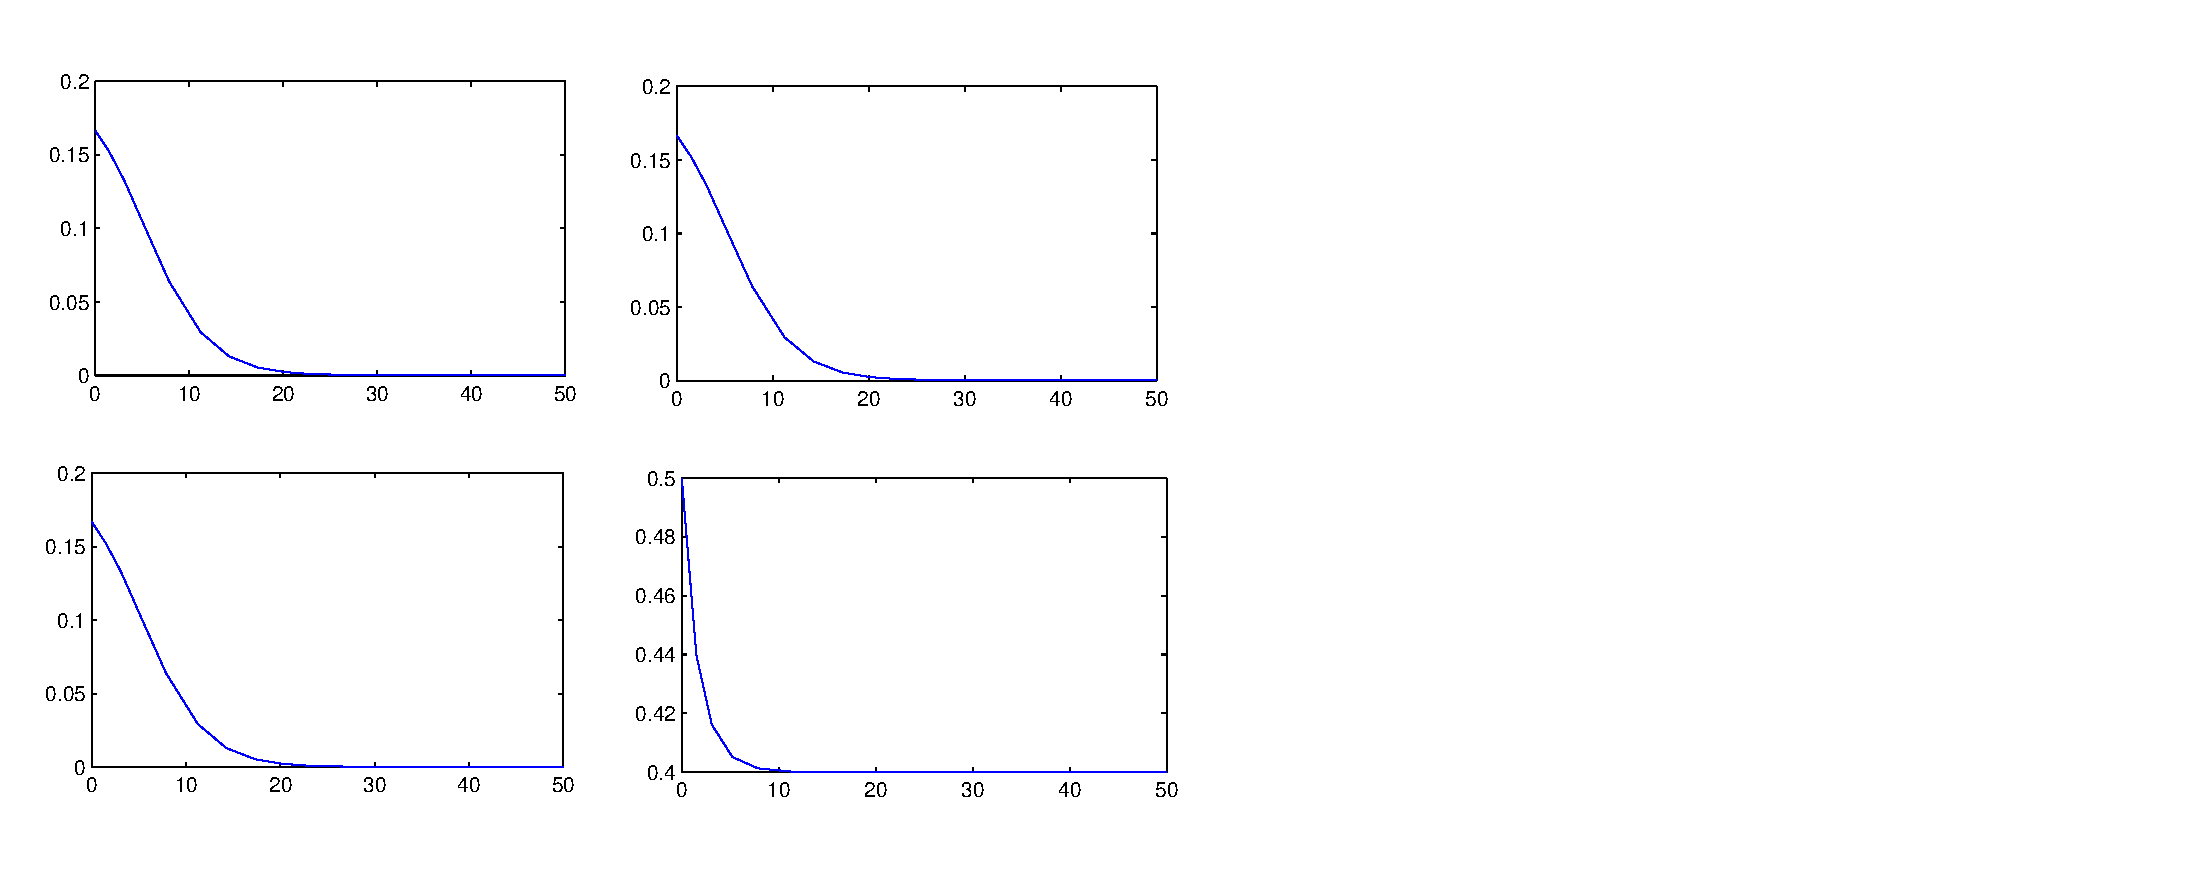
\includegraphics[scale=0.5]{pics/br.eps}
\end{frame}

\begin{frame}{Пример 2}
Начальные условия:
$u_1 = u_2 = 0.2, u_3 = 0.1, u_4 = 0.5$
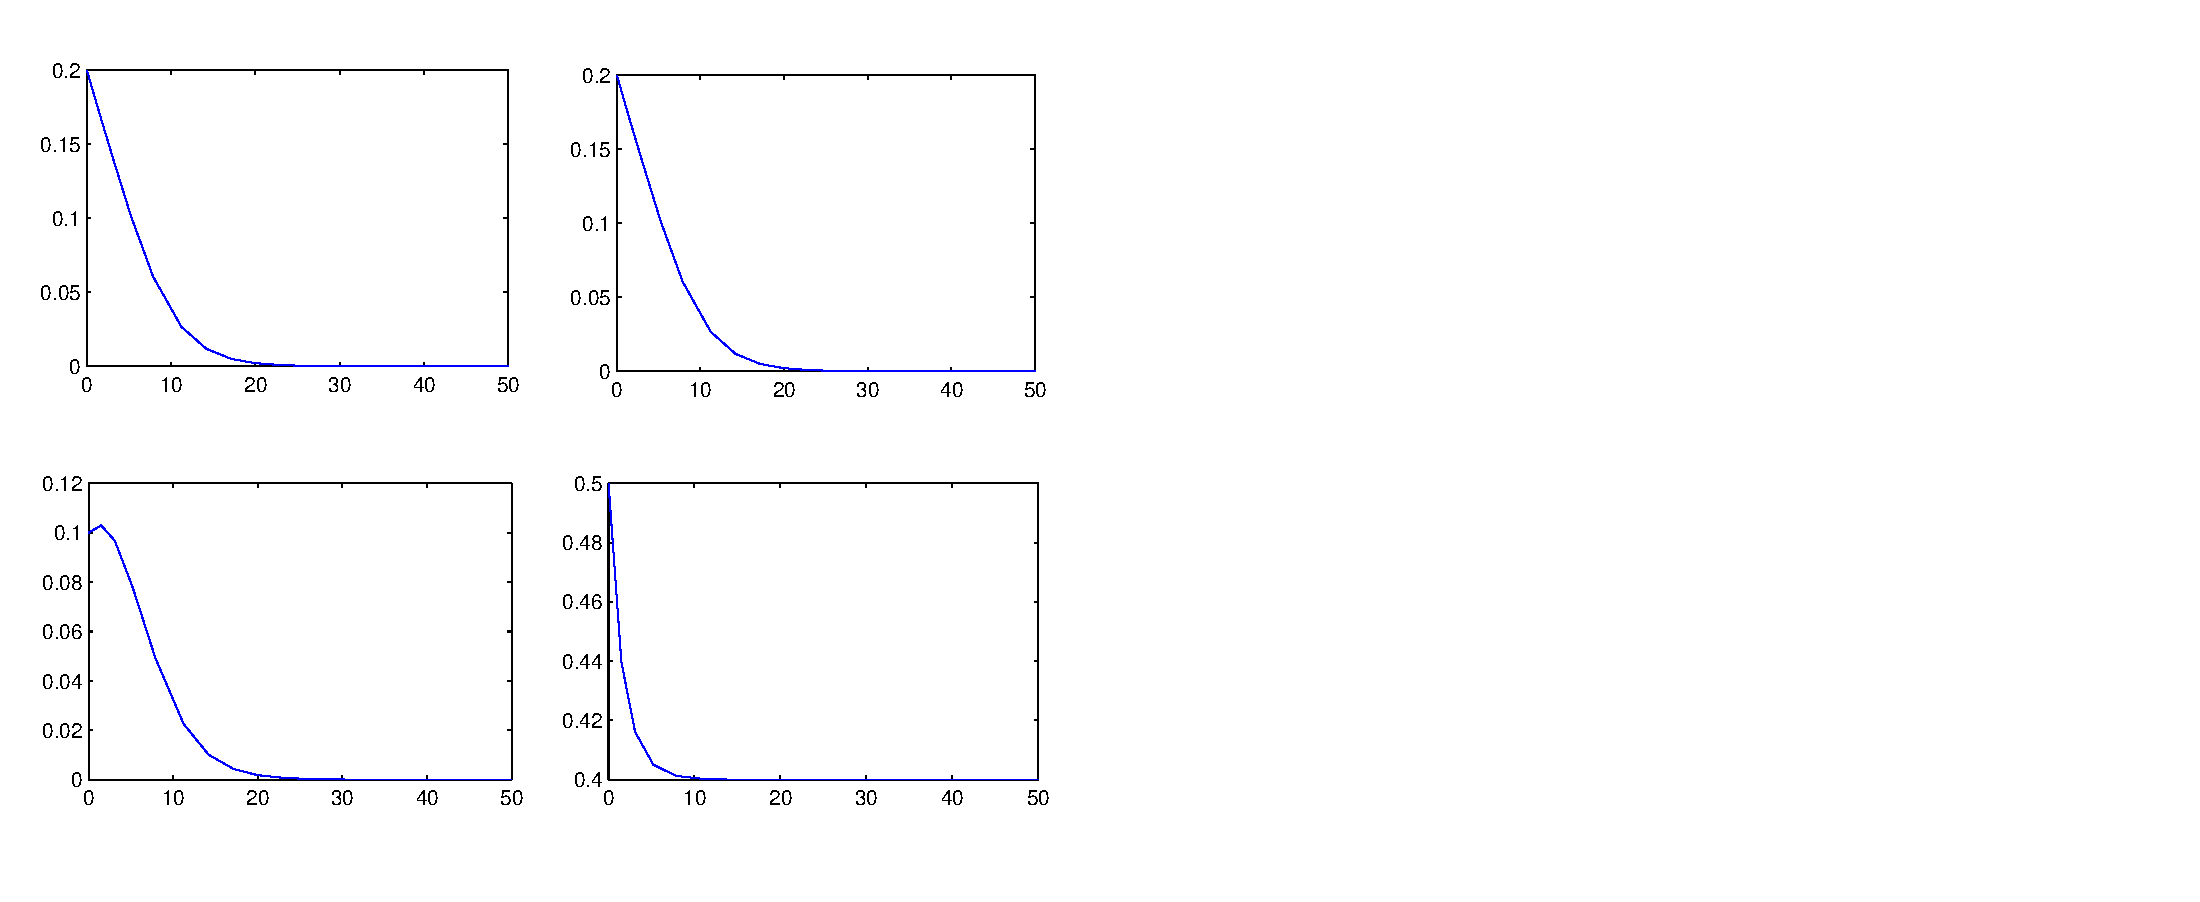
\includegraphics[scale=0.5]{pics/br2.eps}
\end{frame}

\end{document}
